%!TEX root=kapfhammer_gcc_presentation.tex
% mainfile: ../kapfhammer_gcc_presentation.tex

% SLIDE: Table of contents
%!TEX root=kapfhammer_gcc_presentation.tex
% mainfile: ../kapfhammer_gcc_presentation.tex

\begin{frame}

  % \frametitle{\vspace*{.5in}{
  % {\fontsize{22}{0}\selectfont``Searching'' for the Best Tests}}}
  % \framesubtitle{An introduction to automated software testing with search-based techniques}

  \vspace*{.15in}
  \tableofcontents[
  pausesections,
  currentsection,
  % currentsubsection,
  sectionstyle=show/shaded,
  % subsectionstyle=show/shaded,
  ]
\end{frame}



\subsection{Testing Methods}

% SLIDE: Drawbacks of manual testing
%!TEX root=kapfhammer_gatorday2015_presentation.tex
% mainfile: kapfhammer_gatorday2015_presentation.tex

\begin{frame}[t]
  \frametitle{Manual Testing}
  \framesubtitle{While it has benefits, this industry standard may be limited!}

  \hspace*{-.5in}
  \begin{minipage}{5in}
  \begin{center}

    \begin{minipage}{4.5in}

    \tikzstyle{proc} = [draw, thick, fill=solarizedViolet, text centered, rounded corners,
    text=solarizedRebase02, draw=solarizedViolet]

\tikzstyle{prochighlight} = [draw, thick, fill=solarizedOrange, text centered, rounded corners,
    text=solarizedRebase02, draw=solarizedOrange]

\tikzstyle{procold} = [draw, thick, fill=solarizedViolet!75, text centered, rounded corners,
    text=solarizedRebase02, draw=solarizedViolet!75]

\tikzstyle{procchanged} = [draw, thick, fill=solarizedViolet!75, text centered, rounded corners,
    text=solarizedRebase02, draw=solarizedViolet!75]

\tikzstyle{prochighlightold} = [draw, thick, fill=solarizedOrange!75, text centered, rounded corners,
    text=solarizedRebase02, draw=solarizedOrange!75]

\tikzstyle{prochighlightchanged} = [draw, thick, fill=solarizedYellow!75, text centered, rounded corners,
    text=solarizedRebase02, draw=solarizedYellow!75]

\tikzstyle{proctest} = [draw, thick, fill=solarizedOrange, text centered, rounded corners,
text=solarizedBase02, draw=solarizedOrange]

\tikzstyle{procnew} = [draw, thick, fill=solarizedGreen, text centered, rounded corners,
    text=solarizedRebase02, draw=solarizedGreen]

\tikzstyle{procyellow} = [draw, thick, fill=solarizedYellow, text centered, rounded corners,
    text=solarizedRebase02, draw=solarizedYellow]

\tikzstyle{procred} = [draw, thick, fill=solarizedRed, text centered, rounded corners,
    text=solarizedRebase02, draw=solarizedRed]

\tikzstyle{io} = [ellipse, draw, thick, fill=solarizedBlue, draw=solarizedBlue, text=solarizedRebase02]

\tikzstyle{iopass} = [ellipse, draw, thick, fill=solarizedGreen, draw=solarizedGreen, text=solarizedRebase02]
\tikzstyle{iofail} = [ellipse, draw, thick, fill=solarizedRed, draw=solarizedRed, text=solarizedRebase02]
\tikzstyle{iohighlight} = [ellipse, draw, thick, fill=solarizedYellow, draw=solarizedYellow,
    text=solarizedRebase02]

\tikzstyle{iofailother} = [ellipse, draw, thick, fill=solarizedYellow, draw=solarizedYellow,
    text=solarizedRebase02]
\tikzstyle{wrongoutput} = [ellipse, draw, thick, fill=solarizedCyan, draw=solarizedCyan, text=solarizedRebase02]

\tikzstyle{special} = [draw, thick, fill=solarizedGreen, text centered, draw=solarizedGreen,
    text=solarizedBase02]
\tikzstyle{specialOrange} = [draw, thick, fill=solarizedOrange, text centered, draw=solarizedOrange,
    text=solarizedBase02]
\tikzstyle{specialGreen} = [draw, thick, fill=solarizedGreen, text centered, draw=solarizedGreen,
    text=solarizedBase02]
\tikzstyle{specialYellow} = [draw, thick, fill=solarizedYellow, text centered, draw=solarizedYellow,
    text=solarizedBase02]

\tikzstyle{pass} = [draw, thick, fill=solarizedGreen, text centered, draw=solarizedGreen, text=solarizedRebase02]
\tikzstyle{fail} = [draw, thick, fill=solarizedRed, text centered, draw=solarizedRed, text=solarizedRebase02]

\tikzstyle{feature} = [draw, thick, fill=solarizedOrange, text centered, text=solarizedRebase02, draw=solarizedOrange]


    \begin{figure}

    \begin{center}

      \begin{tikzpicture}[node distance=0cm, auto,>=stealth, thick]

        \path[use as bounding box] (-2,4.5) rectangle (10,-2);

        % Computer Software
        \path[->]<1-> node[proc, text width=14ex]
        (Software) at (4,.8) {Manual Testing};

        % Code
        \path[->]<2-> node[proc, right of=Software,
                      yshift=-.5in, xshift=-1.75in, text width=12ex]
                      (Code) {Laborious}
        (Software) edge node {} (Code);

        % Features
        \path[->]<3-> node[proc, below of=Software,
                      yshift=-1in, xshift=-.75in, text width=12ex]
                      (Features) {Time \\ Consuming}
        (Software) edge node {} (Features);

        % Feature Interactions
        \path[->]<4-> node[proc, below of=Software,
                      yshift=-1in, xshift=.75in, text width=12ex]
                      (Interactions) {Very \\ Tedious}
        (Software) edge node {} (Interactions);

        % Execution Environments
        \path[->]<5-> node[proc, right of=Software,
                      yshift=-.5in, xshift=1.75in, text width=12ex]
                      (Environment) {Difficult}
        (Software) edge node {} (Environment);

        % Brooks Quotation
        \path[->]<6-> node[specialOrange, above of=Software,
                      yshift=.8in,text width=40ex]
                      (Quotations)
        {Can we develop and employ methods that will automatically generate high-quality test cases for real-world
        software?};

        \end{tikzpicture}

        \end{center}

        \end{figure}

      \end{minipage}

  \end{center}
  \end{minipage}


\end{frame}



% SLIDE: Benefits of automated testing
%!TEX root=kapfhammer_gcc_presentation.tex
% mainfile: kapfhammer_gcc_presentation.tex

\begin{frame}[t]
  \frametitle{Automated Testing}
  \framesubtitle{Automatically generating tests is amazing --- but does it work?}

  \hspace*{-.5in}
  \begin{minipage}{5in}
  \begin{center}

    \begin{minipage}{4.5in}

    \tikzstyle{proc} = [draw, thick, fill=solarizedViolet, text centered, rounded corners,
    text=solarizedRebase02, draw=solarizedViolet]

\tikzstyle{prochighlight} = [draw, thick, fill=solarizedOrange, text centered, rounded corners,
    text=solarizedRebase02, draw=solarizedOrange]

\tikzstyle{procold} = [draw, thick, fill=solarizedViolet!75, text centered, rounded corners,
    text=solarizedRebase02, draw=solarizedViolet!75]

\tikzstyle{procchanged} = [draw, thick, fill=solarizedViolet!75, text centered, rounded corners,
    text=solarizedRebase02, draw=solarizedViolet!75]

\tikzstyle{prochighlightold} = [draw, thick, fill=solarizedOrange!75, text centered, rounded corners,
    text=solarizedRebase02, draw=solarizedOrange!75]

\tikzstyle{prochighlightchanged} = [draw, thick, fill=solarizedYellow!75, text centered, rounded corners,
    text=solarizedRebase02, draw=solarizedYellow!75]

\tikzstyle{proctest} = [draw, thick, fill=solarizedOrange, text centered, rounded corners,
text=solarizedBase02, draw=solarizedOrange]

\tikzstyle{procnew} = [draw, thick, fill=solarizedGreen, text centered, rounded corners,
    text=solarizedRebase02, draw=solarizedGreen]

\tikzstyle{procyellow} = [draw, thick, fill=solarizedYellow, text centered, rounded corners,
    text=solarizedRebase02, draw=solarizedYellow]

\tikzstyle{procred} = [draw, thick, fill=solarizedRed, text centered, rounded corners,
    text=solarizedRebase02, draw=solarizedRed]

\tikzstyle{io} = [ellipse, draw, thick, fill=solarizedBlue, draw=solarizedBlue, text=solarizedRebase02]

\tikzstyle{iopass} = [ellipse, draw, thick, fill=solarizedGreen, draw=solarizedGreen, text=solarizedRebase02]
\tikzstyle{iofail} = [ellipse, draw, thick, fill=solarizedRed, draw=solarizedRed, text=solarizedRebase02]
\tikzstyle{iohighlight} = [ellipse, draw, thick, fill=solarizedYellow, draw=solarizedYellow,
    text=solarizedRebase02]

\tikzstyle{iofailother} = [ellipse, draw, thick, fill=solarizedYellow, draw=solarizedYellow,
    text=solarizedRebase02]
\tikzstyle{wrongoutput} = [ellipse, draw, thick, fill=solarizedCyan, draw=solarizedCyan, text=solarizedRebase02]

\tikzstyle{special} = [draw, thick, fill=solarizedGreen, text centered, draw=solarizedGreen,
    text=solarizedBase02]
\tikzstyle{specialOrange} = [draw, thick, fill=solarizedOrange, text centered, draw=solarizedOrange,
    text=solarizedBase02]
\tikzstyle{specialGreen} = [draw, thick, fill=solarizedGreen, text centered, draw=solarizedGreen,
    text=solarizedBase02]
\tikzstyle{specialYellow} = [draw, thick, fill=solarizedYellow, text centered, draw=solarizedYellow,
    text=solarizedBase02]

\tikzstyle{pass} = [draw, thick, fill=solarizedGreen, text centered, draw=solarizedGreen, text=solarizedRebase02]
\tikzstyle{fail} = [draw, thick, fill=solarizedRed, text centered, draw=solarizedRed, text=solarizedRebase02]

\tikzstyle{feature} = [draw, thick, fill=solarizedOrange, text centered, text=solarizedRebase02, draw=solarizedOrange]


    \begin{figure}

    \begin{center}

      \begin{tikzpicture}[node distance=0cm, auto,>=stealth, thick]

        \path[use as bounding box] (-2,4.5) rectangle (10,-2);

        % Computer Software
        \path[->]<1-> node[proc, text width=14ex]
        (Software) at (4,.8) {Automated Testing};

        % Code
        \path[->]<2-> node[proc, right of=Software,
                      yshift=-.5in, xshift=-1.75in, text width=12ex]
                      (Code) {Laborious}
        (Software) edge node {} (Code);

        % Features
        \path[->]<3-> node[proc, below of=Software,
                      yshift=-1in, xshift=-.75in, text width=12ex]
                      (Features) {Time \\ Consuming}
        (Software) edge node {} (Features);

        % Feature Interactions
        \path[->]<4-> node[proc, below of=Software,
                      yshift=-1in, xshift=.75in, text width=12ex]
                      (Interactions) {Very \\ Tedious}
        (Software) edge node {} (Interactions);

        % Execution Environments
        \path[->]<5-> node[proc, right of=Software,
                      yshift=-.5in, xshift=1.75in, text width=12ex]
                      (Environment) {Difficult}
        (Software) edge node {} (Environment);

        % Code
        \path[->]<6-> node[procnew, right of=Software,
                      yshift=-.5in, xshift=-1.75in, text width=12ex]
                      (Code) {Laborious}
        (Software) edge node {} (Code);

        % Features
        \path[->]<6-> node[procnew, below of=Software,
                      yshift=-1in, xshift=-.75in, text width=12ex]
                      (Features) {Time \\ Consuming}
        (Software) edge node {} (Features);

        % Feature Interactions
        \path[->]<6-> node[procnew, below of=Software,
                      yshift=-1in, xshift=.75in, text width=12ex]
                      (Interactions) {Very \\ Tedious}
        (Software) edge node {} (Interactions);


        % Brooks Quotation
        \path[->]<6-6> node[specialGreen, above of=Software,
                      yshift=.8in,text width=40ex]
                      (Quotations)
                      {Testing is {\em less} laborious and tedious because an algorithm generates the tests. While computational time is
                      needed, a human can be {\em less} involved!};

        % Code
        \path[->]<7-> node[procnew, right of=Software,
                      yshift=-.5in, xshift=-1.75in, text width=12ex]
                      (Code) {Laborious}
        (Software) edge node {} (Code);

        % Features
        \path[->]<7-> node[procnew, below of=Software,
                      yshift=-1in, xshift=-.75in, text width=12ex]
                      (Features) {Time \\ Consuming}
        (Software) edge node {} (Features);

        % Feature Interactions
        \path[->]<7-> node[procnew, below of=Software,
                      yshift=-1in, xshift=.75in, text width=12ex]
                      (Interactions) {Very \\ Tedious}
        (Software) edge node {} (Interactions);

        % Execution Environments
        \path[->]<7-> node[procyellow, right of=Software,
                      yshift=-.5in, xshift=1.75in, text width=12ex]
                      (Environment) {Difficult}
        (Software) edge node {} (Environment);

        % Brooks Quotation
        \path[->]<7-> node[specialYellow, above of=Software,
                      yshift=.8in,text width=40ex]
                      (Quotations)
                      {Automated testing is {\em less} difficult since a good fitness function can guide the algorithm to inputs that find
        the faults};

        \end{tikzpicture}

        \end{center}

        \end{figure}

      \end{minipage}

  \end{center}
  \end{minipage}


\end{frame}



\subsection{Random Testing}

% SLIDE: Introduction Random Testing
%!TEX root=kapfhammer_gcc_presentation.tex
% mainfile: ../kapfhammer_gcc_presentation.tex

\begin{frame}[t]

  \frametitle{Random Testing}
  \framesubtitle{It is easy to randomly generate tests --- but how good are they?}

  \vspace*{.2in}
  \hspace{.4in}
  \resizebox{3.0in}{!}{
    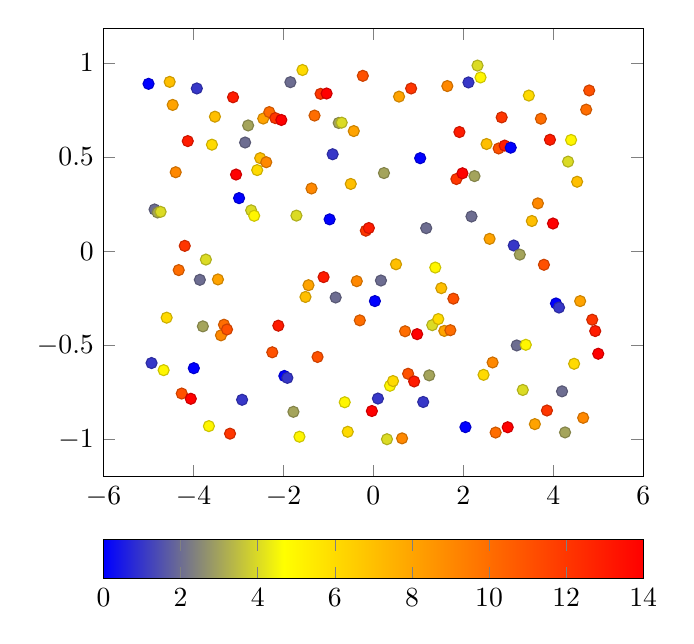
\begin{tikzpicture}
      \begin{axis}[colorbar horizontal]
        \addplot[only marks,scatter,
          scatter src={mod(\coordindex,15)},samples=150]
          {rand};
      \end{axis}
  \end{tikzpicture}}

\end{frame}


\subsection{Testing with EvoSuite}

% SLIDE: Introduction SBST Testing
%!TEX root=kapfhammer_gatorday2015_presentation.tex
% mainfile: ../kapfhammer_gatorday2015_presentation.tex

\begin{frame}[t]

  \frametitle{Search-Based Testing}
  \framesubtitle{Use a fitness function to guide the search to ``good'' values}

  \vspace*{.25in}
  \hspace{.25in}
  \resizebox{3.5in}{!}{
    \begin{tikzpicture}
      \begin{axis}[
          domain=0:1,
          xmax=1,
          ymax=1,
        ]
        \addplot3[surf] {x*y};
        \addplot3[solarizedRebase0,/pgfplots/quiver,
            quiver/u=y,
            quiver/v=x,
            quiver/w=0,
            quiver/scale arrows=0.1,
          -stealth,samples=10] {1};
      \end{axis}
  \end{tikzpicture}}

\end{frame}


% SLIDE: Introduction Mutation Testing
%!TEX root=kapfhammer_gcc_presentation.tex
% mainfile: ../kapfhammer_gcc_presentation.tex

\begin{frame}[t]

  \frametitle{Mutation Testing}
  \framesubtitle{Let's purposefully insert faults into the program under test!}


  \hspace*{-.5in}
  \begin{minipage}{5in}
  \begin{center}

    \begin{minipage}{4.5in}
      \tikzstyle{proc} = [draw, thick, fill=solarizedViolet, text centered, rounded corners,
    text=solarizedRebase02, draw=solarizedViolet]

\tikzstyle{prochighlight} = [draw, thick, fill=solarizedOrange, text centered, rounded corners,
    text=solarizedRebase02, draw=solarizedOrange]

\tikzstyle{procold} = [draw, thick, fill=solarizedViolet!75, text centered, rounded corners,
    text=solarizedRebase02, draw=solarizedViolet!75]

\tikzstyle{procchanged} = [draw, thick, fill=solarizedViolet!75, text centered, rounded corners,
    text=solarizedRebase02, draw=solarizedViolet!75]

\tikzstyle{prochighlightold} = [draw, thick, fill=solarizedOrange!75, text centered, rounded corners,
    text=solarizedRebase02, draw=solarizedOrange!75]

\tikzstyle{prochighlightchanged} = [draw, thick, fill=solarizedYellow!75, text centered, rounded corners,
    text=solarizedRebase02, draw=solarizedYellow!75]

\tikzstyle{proctest} = [draw, thick, fill=solarizedOrange, text centered, rounded corners,
text=solarizedBase02, draw=solarizedOrange]

\tikzstyle{procnew} = [draw, thick, fill=solarizedGreen, text centered, rounded corners,
    text=solarizedRebase02, draw=solarizedGreen]

\tikzstyle{procyellow} = [draw, thick, fill=solarizedYellow, text centered, rounded corners,
    text=solarizedRebase02, draw=solarizedYellow]

\tikzstyle{procred} = [draw, thick, fill=solarizedRed, text centered, rounded corners,
    text=solarizedRebase02, draw=solarizedRed]

\tikzstyle{io} = [ellipse, draw, thick, fill=solarizedBlue, draw=solarizedBlue, text=solarizedRebase02]

\tikzstyle{iopass} = [ellipse, draw, thick, fill=solarizedGreen, draw=solarizedGreen, text=solarizedRebase02]
\tikzstyle{iofail} = [ellipse, draw, thick, fill=solarizedRed, draw=solarizedRed, text=solarizedRebase02]
\tikzstyle{iohighlight} = [ellipse, draw, thick, fill=solarizedYellow, draw=solarizedYellow,
    text=solarizedRebase02]

\tikzstyle{iofailother} = [ellipse, draw, thick, fill=solarizedYellow, draw=solarizedYellow,
    text=solarizedRebase02]
\tikzstyle{wrongoutput} = [ellipse, draw, thick, fill=solarizedCyan, draw=solarizedCyan, text=solarizedRebase02]

\tikzstyle{special} = [draw, thick, fill=solarizedGreen, text centered, draw=solarizedGreen,
    text=solarizedBase02]
\tikzstyle{specialOrange} = [draw, thick, fill=solarizedOrange, text centered, draw=solarizedOrange,
    text=solarizedBase02]
\tikzstyle{specialGreen} = [draw, thick, fill=solarizedGreen, text centered, draw=solarizedGreen,
    text=solarizedBase02]
\tikzstyle{specialYellow} = [draw, thick, fill=solarizedYellow, text centered, draw=solarizedYellow,
    text=solarizedBase02]

\tikzstyle{pass} = [draw, thick, fill=solarizedGreen, text centered, draw=solarizedGreen, text=solarizedRebase02]
\tikzstyle{fail} = [draw, thick, fill=solarizedRed, text centered, draw=solarizedRed, text=solarizedRebase02]

\tikzstyle{feature} = [draw, thick, fill=solarizedOrange, text centered, text=solarizedRebase02, draw=solarizedOrange]


    \begin{figure}

    \begin{center}

      \begin{tikzpicture}[node distance=1cm, auto,>=stealth, thick]

        \path[use as bounding box] (-2,4.35) rectangle (10,-2);

%% 10 test cases, 12 requirements
%% Test case timings (used by Greedy): 5,6,4,2,8,10,4,1,3,2
%% Covers relationships:
%%   T1 = {R1,R2,R3}
%%   T2 = {R2,R3,R4}
%%   T3 = {R1,R5}
%%   T4 = {R4,R6}
%%   T5 = {R5,R6,R7}
%%   T6 = {R6,R7,R8,R9}
%%   T7 = {R7,R8}
%%   T8 = {R8,R10}
%%   T9 = {R9,R12}
%%   T10 = {R10,R11}

        %%%%% 1

        % A Test Case
        \path[->]<1-> node[proc, text width=3ex]
        (One) at (-1.65,2.00) {$T_1$};

        % A Test Case
        \path[->]<1-> node[proc, right of=One,
                      yshift=0in, xshift=.1in, text width=3ex]
                      (Two) {$T_2$};

        % A Test Case
        \path[->]<2-> node[proc, right of=Two,
                      yshift=0in, xshift=.1in, text width=3ex]
                      (Three) {$T_3$};

        % A Test Case
        \path[->]<2-> node[proc, right of=Three,
                      yshift=0in, xshift=.1in, text width=3ex]
                      (Four) {$T_4$};

        % A Test Case
        \path[->]<3-> node[proc, right of=Four,
                      yshift=0in, xshift=.1in, text width=3ex]
                      (Five) {$T_5$};

        % A Test Case
        \path[->]<3-> node[proc, right of=Five,
                      yshift=0in, xshift=.1in, text width=3ex]
                      (Six) {$T_6$};

        % A Test Case
        \path[->]<4-> node[proc, right of=Six,
                      yshift=0in, xshift=.1in, text width=3ex]
                      (Seven) {$T_7$};

        % A Test Case
        \path[->]<4-> node[proc, right of=Seven,
                      yshift=0in, xshift=.1in, text width=3ex]
                      (Eight) {$T_8$};

        % A Test Case
        \path[->]<5-> node[proc, right of=Eight,
                      yshift=0in, xshift=.1in, text width=3ex]
                      (Nine) {$T_9$};

        % A Test Case
        \path[->]<5-> node[proc, right of=Nine,
                      yshift=0in, xshift=.1in, text width=3ex]
                      (Ten) {$T_{10}$};

        % Show the test suite
        \path[->]<6-> node[special, above of=Five,
                      yshift=.1in, xshift=.25in]
                      (TestSuite)
              {Test Suite $T = \langle T_1, T_2, \ldots, T_9, T_{10} \rangle$};

%% 10 test cases, 12 requirements
%% Test case timings (used by Greedy): 5,6,4,2,8,10,4,1,3,2
%% Covers relationships:
%%   T1 = {R1,R2,R3}
%%   T2 = {R2,R3,R4}
%%   T3 = {R1,R5}
%%   T4 = {R4,R6}
%%   T5 = {R5,R6,R7}
%%   T6 = {R6,R7,R8,R9}
%%   T7 = {R7,R8}
%%   T8 = {R8,R10}
%%   T9 = {R9,R12}
%%   T10 = {R10,R11}

        %%%%% 2

        \path[->]<7-> node[prochighlight, text width=3ex]
        (OneR) at (-1.825,-1.00) {$M_1$};

        \path[->]<7-> node[prochighlight, right of=OneR,
                      yshift=0in, xshift=.02in, text width=3ex]
                      (TwoR) {$M_2$};

        \path[->]<8-> node[prochighlight, right of=TwoR,
                      yshift=0in, xshift=.02in, text width=3ex]
                      (ThreeR) {$M_3$};

        \path[->]<8-> node[prochighlight, right of=ThreeR,
                      yshift=0in, xshift=.02in, text width=3ex]
                      (FourR) {$M_4$};

        \path[->]<9-> node[prochighlight, right of=FourR,
                      yshift=0in, xshift=.02in, text width=3ex]
                      (FiveR) {$M_5$};

        \path[->]<9-> node[prochighlight, right of=FiveR,
                      yshift=0in, xshift=.02in, text width=3ex]
                      (SixR) {$M_6$};

        \path[->]<10-> node[prochighlight, right of=SixR,
                      yshift=0in, xshift=.02in, text width=3ex]
                      (SevenR) {$M_7$};

        \path[->]<10-> node[prochighlight, right of=SevenR,
                      yshift=0in, xshift=.02in, text width=3ex]
                      (EightR) {$M_8$};

        \path[->]<11-> node[prochighlight, right of=EightR,
                      yshift=0in, xshift=.02in, text width=3ex]
                      (NineR) {$M_9$};

        \path[->]<11-> node[prochighlight, right of=NineR,
                      yshift=0in, xshift=.02in, text width=3ex]
                      (TenR) {$M_{10}$};

        \path[->]<12-> node[prochighlight, right of=TenR,
                      yshift=0in, xshift=.02in, text width=3ex]
                      (ElevenR) {$M_{11}$};

        \path[->]<12-> node[prochighlight, right of=ElevenR,
                      yshift=0in, xshift=.02in, text width=3ex]
                      (TwelveR) {$M_{12}$};

%% 10 test cases, 12 requirements
%% Test case timings (used by Greedy): 5,6,4,2,8,10,4,1,3,2
%% Covers relationships:
%%   T1 = {R1,R2,R3}
%%   T2 = {R2,R3,R4}
%%   T3 = {R1,R5}
%%   T4 = {R4,R6}
%%   T5 = {R5,R6,R7}
%%   T6 = {R6,R7,R8,R9}
%%   T7 = {R7,R8}
%%   T8 = {R8,R10}
%%   T9 = {R9,R12}
%%   T10 = {R10,R11}

        %%%%% 3

        % Show the set of requirements
        \path[->]<13-> node[special, below of=SixR,
                      yshift=-.1in, xshift=.25in]
                      (Requirements)
              {Set of Program Methods $M = \{ M_1, M_2, \ldots, M_{11}, M_{12} \}$};

        %%%%% 4

        \path[->]<14-> node[prochighlight, right of=ElevenR,
                      yshift=0in, xshift=.02in, text width=3ex]
                      (TwelveR) {$M_{12}$}
        (One) edge node {} (OneR)
        (One) edge node {} (TwoR)
        (One) edge node {} (FourR);

        \path[->]<14-> node[prochighlight, right of=ElevenR,
                      yshift=0in, xshift=.02in, text width=3ex]
                      (TwelveR) {$M_{12}$}
        (Two) edge node {} (TwoR)
        (Two) edge node {} (ThreeR)
        (Two) edge node {} (FourR);

        \path[->]<14-> node[prochighlight, right of=ElevenR,
                      yshift=0in, xshift=.02in, text width=3ex]
                      (TwelveR) {$M_{12}$}
        (Three) edge node {} (OneR)
        (Three) edge node {} (FiveR);

        \path[->]<14-> node[prochighlight, right of=ElevenR,
                      yshift=0in, xshift=.02in, text width=3ex]
                      (TwelveR) {$M_{12}$}
        (Four) edge node {} (FourR)
        (Four) edge node {} (SixR);

        \path[->]<15-> node[prochighlight, right of=ElevenR,
                      yshift=0in, xshift=.02in, text width=3ex]
                      (TwelveR) {$M_{12}$}
        (Five) edge node {} (FiveR)
        (Five) edge node {} (SixR)
        (Five) edge node {} (SevenR);

        \path[->]<15-> node[prochighlight, right of=ElevenR,
                      yshift=0in, xshift=.02in, text width=3ex]
                      (TwelveR) {$M_{12}$}
        (Six) edge node {} (SixR)
        (Six) edge node {} (SevenR)
        (Six) edge node {} (EightR)
        (Six) edge node {} (NineR);

        \path[->]<16-> node[prochighlight, right of=ElevenR,
                      yshift=0in, xshift=.02in, text width=3ex]
                      (TwelveR) {$M_{12}$}
        (Seven) edge node {} (SevenR)
        (Seven) edge node {} (EightR);

        \path[->]<16-> node[prochighlight, right of=ElevenR,
                      yshift=0in, xshift=.02in, text width=3ex]
                      (TwelveR) {$M_{12}$}
        (Eight) edge node {} (EightR)
        (Eight) edge node {} (TenR);

        \path[->]<16-> node[prochighlight, right of=ElevenR,
                      yshift=0in, xshift=.02in, text width=3ex]
                      (TwelveR) {$M_{12}$}
        (Nine) edge node {} (NineR)
        (Nine) edge node {} (TwelveR);

        \path[->]<16-> node[prochighlight, right of=ElevenR,
                      yshift=0in, xshift=.02in, text width=3ex]
                      (TwelveR) {$M_{12}$}
        (Ten) edge node {} (TenR)
        (Ten) edge node {} (ElevenR);

        % FINAL PART WHERE WE EITHER FIND OR DO NOT FIND THE FAULT

        \path[->]<17-18> node[procyellow, right of=ThreeR,
                      yshift=0in, xshift=.02in, text width=3ex]
                      (FourR) {$M_4$};

        % A Test Case
        \path[->]<18-18> node[procred, text width=3ex]
        (One) at (-1.65,2.00) {$T_1$};

        \path[->]<19-> node[prochighlight, right of=ThreeR,
                      yshift=0in, xshift=.02in, text width=3ex]
                      (FourR) {$M_4$};

        % A Test Case
        \path[->]<19-> node[proc, text width=3ex]
        (One) at (-1.65,2.00) {$T_1$};

        \path[->]<20-> node[procyellow, right of=SevenR,
                      yshift=0in, xshift=.02in, text width=3ex]
                      (EightR) {$M_8$};

        \end{tikzpicture}

        \end{center}

        \end{figure}

      \end{minipage}

  \end{center}
  \end{minipage}

\end{frame}


% SLIDE: Explain the basics of EvoSuite
%!TEX root=kapfhammer_gatorday2015_presentation.tex
% mainfile: kapfhammer_gatorday2015_presentation.tex

\begin{frame}[t]
  \frametitle{Testing with EvoSuite}
  \framesubtitle{This prototype can automatically generate real JUnit test suites!}

  \hspace*{-.5in}
  \begin{minipage}{5in}
  \begin{center}

    \begin{minipage}{4.5in}

    \tikzstyle{proc} = [draw, thick, fill=solarizedViolet, text centered, rounded corners,
    text=solarizedRebase02, draw=solarizedViolet]

\tikzstyle{prochighlight} = [draw, thick, fill=solarizedOrange, text centered, rounded corners,
    text=solarizedRebase02, draw=solarizedOrange]

\tikzstyle{procold} = [draw, thick, fill=solarizedViolet!75, text centered, rounded corners,
    text=solarizedRebase02, draw=solarizedViolet!75]

\tikzstyle{procchanged} = [draw, thick, fill=solarizedViolet!75, text centered, rounded corners,
    text=solarizedRebase02, draw=solarizedViolet!75]

\tikzstyle{prochighlightold} = [draw, thick, fill=solarizedOrange!75, text centered, rounded corners,
    text=solarizedRebase02, draw=solarizedOrange!75]

\tikzstyle{prochighlightchanged} = [draw, thick, fill=solarizedYellow!75, text centered, rounded corners,
    text=solarizedRebase02, draw=solarizedYellow!75]

\tikzstyle{proctest} = [draw, thick, fill=solarizedOrange, text centered, rounded corners,
text=solarizedBase02, draw=solarizedOrange]

\tikzstyle{procnew} = [draw, thick, fill=solarizedGreen, text centered, rounded corners,
    text=solarizedRebase02, draw=solarizedGreen]

\tikzstyle{procyellow} = [draw, thick, fill=solarizedYellow, text centered, rounded corners,
    text=solarizedRebase02, draw=solarizedYellow]

\tikzstyle{procred} = [draw, thick, fill=solarizedRed, text centered, rounded corners,
    text=solarizedRebase02, draw=solarizedRed]

\tikzstyle{io} = [ellipse, draw, thick, fill=solarizedBlue, draw=solarizedBlue, text=solarizedRebase02]

\tikzstyle{iopass} = [ellipse, draw, thick, fill=solarizedGreen, draw=solarizedGreen, text=solarizedRebase02]
\tikzstyle{iofail} = [ellipse, draw, thick, fill=solarizedRed, draw=solarizedRed, text=solarizedRebase02]
\tikzstyle{iohighlight} = [ellipse, draw, thick, fill=solarizedYellow, draw=solarizedYellow,
    text=solarizedRebase02]

\tikzstyle{iofailother} = [ellipse, draw, thick, fill=solarizedYellow, draw=solarizedYellow,
    text=solarizedRebase02]
\tikzstyle{wrongoutput} = [ellipse, draw, thick, fill=solarizedCyan, draw=solarizedCyan, text=solarizedRebase02]

\tikzstyle{special} = [draw, thick, fill=solarizedGreen, text centered, draw=solarizedGreen,
    text=solarizedBase02]
\tikzstyle{specialOrange} = [draw, thick, fill=solarizedOrange, text centered, draw=solarizedOrange,
    text=solarizedBase02]
\tikzstyle{specialGreen} = [draw, thick, fill=solarizedGreen, text centered, draw=solarizedGreen,
    text=solarizedBase02]
\tikzstyle{specialYellow} = [draw, thick, fill=solarizedYellow, text centered, draw=solarizedYellow,
    text=solarizedBase02]

\tikzstyle{pass} = [draw, thick, fill=solarizedGreen, text centered, draw=solarizedGreen, text=solarizedRebase02]
\tikzstyle{fail} = [draw, thick, fill=solarizedRed, text centered, draw=solarizedRed, text=solarizedRebase02]

\tikzstyle{feature} = [draw, thick, fill=solarizedOrange, text centered, text=solarizedRebase02, draw=solarizedOrange]


    \begin{figure}

    \begin{center}

      \begin{tikzpicture}[node distance=0cm, auto,>=stealth, thick]

        \path[use as bounding box] (-2,4.5) rectangle (10,-2);

        % Computer Software
        \path[->]<1-> node[proc, text width=14ex]
        (Software) at (4,.8) {Evolutionary Testing};

        % Code
        \path[->]<2-> node[proc, right of=Software,
                      yshift=-.5in, xshift=-1.75in, text width=14ex]
                      (Code) {Representation}
        (Software) edge node {} (Code);

        % Features
        \path[->]<3-> node[proc, below of=Software,
                      yshift=-1in, xshift=-.75in, text width=12ex]
                      (Features) {Fitness \\ Function}
        (Software) edge node {} (Features);

        % Feature Interactions
        \path[->]<4-> node[proc, below of=Software,
                      yshift=-1in, xshift=.75in, text width=12ex]
                      (Interactions) {Modify \\ Program}
        (Software) edge node {} (Interactions);

        % Execution Environments
        \path[->]<5-> node[proc, right of=Software,
                      yshift=-.5in, xshift=1.75in, text width=12ex]
                      (Environment) {Operators}
        (Software) edge node {} (Environment);

        % Brooks Quotation
        \path[->]<6-> node[specialOrange, above of=Software,
                      yshift=.8in,text width=40ex]
                      (Quotations)
                      {``1600 Faults in 100 Projects: Automatically Finding Faults While Achieving High Coverage with
                      EvoSuite'', {\em Empirical Software Engineering}};

        \end{tikzpicture}

        \end{center}

        \end{figure}

      \end{minipage}

  \end{center}
  \end{minipage}


\end{frame}



% SLIDE: Explain the EvoSuite methods
%!TEX root=kapfhammer_gatorday2015_presentation.tex
% mainfile: kapfhammer_gatorday2015_presentation.tex

\begin{frame}[t]
  \frametitle{Configuring EvoSuite}
  \framesubtitle{This tool has many unique configurations --- which are best?}

  \hspace*{-.5in}
  \begin{minipage}{5in}
  \begin{center}
  \vspace*{.1in}

    \begin{minipage}{4.5in}

    \tikzstyle{proc} = [draw, thick, fill=solarizedViolet, text centered, rounded corners,
    text=solarizedRebase02, draw=solarizedViolet]

\tikzstyle{prochighlight} = [draw, thick, fill=solarizedOrange, text centered, rounded corners,
    text=solarizedRebase02, draw=solarizedOrange]

\tikzstyle{procold} = [draw, thick, fill=solarizedViolet!75, text centered, rounded corners,
    text=solarizedRebase02, draw=solarizedViolet!75]

\tikzstyle{procchanged} = [draw, thick, fill=solarizedViolet!75, text centered, rounded corners,
    text=solarizedRebase02, draw=solarizedViolet!75]

\tikzstyle{prochighlightold} = [draw, thick, fill=solarizedOrange!75, text centered, rounded corners,
    text=solarizedRebase02, draw=solarizedOrange!75]

\tikzstyle{prochighlightchanged} = [draw, thick, fill=solarizedYellow!75, text centered, rounded corners,
    text=solarizedRebase02, draw=solarizedYellow!75]

\tikzstyle{proctest} = [draw, thick, fill=solarizedOrange, text centered, rounded corners,
text=solarizedBase02, draw=solarizedOrange]

\tikzstyle{procnew} = [draw, thick, fill=solarizedGreen, text centered, rounded corners,
    text=solarizedRebase02, draw=solarizedGreen]

\tikzstyle{procyellow} = [draw, thick, fill=solarizedYellow, text centered, rounded corners,
    text=solarizedRebase02, draw=solarizedYellow]

\tikzstyle{procred} = [draw, thick, fill=solarizedRed, text centered, rounded corners,
    text=solarizedRebase02, draw=solarizedRed]

\tikzstyle{io} = [ellipse, draw, thick, fill=solarizedBlue, draw=solarizedBlue, text=solarizedRebase02]

\tikzstyle{iopass} = [ellipse, draw, thick, fill=solarizedGreen, draw=solarizedGreen, text=solarizedRebase02]
\tikzstyle{iofail} = [ellipse, draw, thick, fill=solarizedRed, draw=solarizedRed, text=solarizedRebase02]
\tikzstyle{iohighlight} = [ellipse, draw, thick, fill=solarizedYellow, draw=solarizedYellow,
    text=solarizedRebase02]

\tikzstyle{iofailother} = [ellipse, draw, thick, fill=solarizedYellow, draw=solarizedYellow,
    text=solarizedRebase02]
\tikzstyle{wrongoutput} = [ellipse, draw, thick, fill=solarizedCyan, draw=solarizedCyan, text=solarizedRebase02]

\tikzstyle{special} = [draw, thick, fill=solarizedGreen, text centered, draw=solarizedGreen,
    text=solarizedBase02]
\tikzstyle{specialOrange} = [draw, thick, fill=solarizedOrange, text centered, draw=solarizedOrange,
    text=solarizedBase02]
\tikzstyle{specialGreen} = [draw, thick, fill=solarizedGreen, text centered, draw=solarizedGreen,
    text=solarizedBase02]
\tikzstyle{specialYellow} = [draw, thick, fill=solarizedYellow, text centered, draw=solarizedYellow,
    text=solarizedBase02]

\tikzstyle{pass} = [draw, thick, fill=solarizedGreen, text centered, draw=solarizedGreen, text=solarizedRebase02]
\tikzstyle{fail} = [draw, thick, fill=solarizedRed, text centered, draw=solarizedRed, text=solarizedRebase02]

\tikzstyle{feature} = [draw, thick, fill=solarizedOrange, text centered, text=solarizedRebase02, draw=solarizedOrange]


    \begin{figure}

    \begin{center}

      \begin{tikzpicture}[node distance=0cm, auto,>=stealth, thick]

        \path[use as bounding box] (-2,4.5) rectangle (10,-2);

        % Computer Software
        \path[->]<1-> node[proc, text width=14ex]
        (Software) at (4,.8) {EvoSuite's Configurations};

        % Code
        \path[->]<2-> node[proc, right of=Software,
                      yshift=-.5in, xshift=-1.75in, text width=12ex]
                      (Code) {Random}
        (Software) edge node {} (Code);

        % Features
        \path[->]<3-> node[proc, below of=Software,
                      yshift=-1in, xshift=-.75in, text width=14ex]
                      (Features) {Fixed-Random}
        (Software) edge node {} (Features);

        % Feature Interactions
        \path[->]<4-> node[proc, below of=Software,
                      yshift=-1in, xshift=.75in, text width=12ex]
                      (Interactions) {Genetic}
        (Software) edge node {} (Interactions);

        % Execution Environments
        \path[->]<5-> node[proc, right of=Software,
                      yshift=-.5in, xshift=1.75in, text width=12ex]
                      (Environment) {Regression}
        (Software) edge node {} (Environment);

        % Brooks Quotation
        \path[->]<6-> node[specialOrange, above of=Software,
                      yshift=.8in,text width=40ex]
                      (Quotations)
                      {The fitness function computes {\em branch coverage}, {\em weak mutation score}, or {\em strong
                      mutation score} to guide the search to the ``best'' test cases};

        \end{tikzpicture}

        \end{center}

        \end{figure}

      \end{minipage}

  \end{center}
  \end{minipage}


\end{frame}



% SLIDE: Show a Test Case Generated by EvoSuite
%!TEX root=kapfhammer_gcc_presentation.tex
% mainfile: ../kapfhammer_gcc_presentation.tex

\begin{frame}[fragile]
  \frametitle{\vspace*{.5in}A Test from EvoSuite}
  \framesubtitle{}

  \normalsize
  \hspace*{-.75in}
  \begin{minipage}{5in}
    \large
    \vspace*{-.25in}
    \begin{minted}{java}

      @Test
      public void test001() throws Throwable {
        int int0 = 0;
        String string0 = Kinetic.computeVelocity(int0, int0);
        assertEquals("Undefined", string0);
        assertNotNull(string0);
        int int1 = 1262;
        String string1 = Kinetic.computeVelocity(int0, int0);
        int int2 = 5349;
        String string2 = Kinetic.computeVelocity(int1, int2);
        int int3 = 0;
        int int4 = 3;
        String string3 = Kinetic.computeVelocity(int3, int4);
        Kinetic kinetic0 = new Kinetic();
      }

    \end{minted}
  \end{minipage}
  \normalsize

\end{frame}


% SLIDE: Ask some questions about the use of EvoSuite
%!TEX root=kapfhammer_gcc_presentation.tex
% mainfile: ../kapfhammer_gcc_presentation.tex

\begin{frame}[t]

  \frametitle{Important Questions}
  \framesubtitle{EvoSuite is an advanced, yet sometimes limited, testing tool}

  \begin{tikzpicture}[overlay, remember picture]
    \node[anchor=center] at (current page.center) {
        \begin{beamercolorbox}[center]{title}
          \vspace*{.4in}
          \fontsize{30}{40}\selectfont
          \begin{center}
            \only<1>{\vspace*{.2in} Will EvoSuite's test cases find the fault in the example program?}
            \only<2>{What is missing from the test cases that EvoSuite generates?}
            \only<3>{\vspace*{.2in}How does the {\em oracle problem} influence the effectiveness of EvoSuite?}
            \only<4>{\vspace*{.2in}What are the {\em fundamental} limitations of automated testing?}
          \end{center}
          \normalsize
      \end{beamercolorbox}};
  \end{tikzpicture}

\end{frame}


% SLIDE: Introduce the NSB hypothesis
%!TEX root=kapfhammer_gatorday2015_presentation.tex
% mainfile: ../kapfhammer_gatorday2015_presentation.tex

\begin{frame}[t]

  \frametitle{No Silver Bullet}
  \framesubtitle{Software tools are fundamentally limited --- what is our hope?}

  \begin{tikzpicture}[overlay, remember picture]
    \node[anchor=center] at (current page.center) {
        \begin{beamercolorbox}[center]{title}
          \vspace*{.8in}
          \Large
          \begin{center}
            \begin{quote}
              There is no single development, in either technology or management technique, which by itself promises even
              one order-of-magnitude improvement within a decade in productivity, in reliability, in simplicity. \\ \vspace*{.1in}
              {\color{solarizedViolet}{\em Frederick P.\ Brooks, Jr.}, Proceedings of the IFIP Tenth World Computing
              Conference, {\em 1986}}
            \end{quote}
          \end{center}
          \normalsize
      \end{beamercolorbox}};
  \end{tikzpicture}

\end{frame}












